\section{GenetischerAlgorithmus}
\label{sec:GenetischerAlgorithmus}
Das nachfolgende Kapitel stellt den genetischen Algorithmus, als Verfahren zur Lösung komplexer Optimierungsprobleme, vor. Dazu werden im ersten Schritt die benötigten Grundlagen geschaffen und im Anschluss die speziellen Operatoren im Zusammenhang mit dem "`PDPTW"' vorgestellt. 

\subsection{Grundlagen}
Bei den genetischen Algorithmen handelt es sich um Verfahren, die zur Lösung komplexer Optimierungsaufgaben eingesetzt werden. Sie beruhen auf Methoden und Erkenntnisse der biologischen Genetik. Dabei dient insbesondere die Evolutionstheorie als Vorbild für die Entwicklung der genetischen Algorithmen, da die Evolution bislang gute Ergebnisse in der Natur geliefert hat. \cite{jih2004family} \cite{bortfeldtplanen}

Die grundlegende Arbeit, zur Schaffung dieser Verfahrenstechnik, wurde von I. Rechenberg mit dem 1960 erschienenen Werk "`Evolutionsstrategie"' geschaffen. Auf diesem Wissen aufbauend, erfand John Holland 1975 die genetischen Algorithmen, die in seinem Werk "`Adaption in Natural and Artificial Systems"' niedergeschrieben wurden.

Der genetische Algorithmus beruht dabei auf eine simple Verfahrenstechnik, welche nachfolgend dargestellt und erklärt wird:
\begin{itemize}
 \item Initialisiere Population P
 \item Evaluiere alle Individuen in P
 \item Wiederhole, solange Abbruchbedingung nicht erreicht
 \begin{itemize}
  \item Selektiere ein Individuenpaar x, y aus P als Eltern
  \item Erzeuge zwei Nachkommen x‘, y‘ aus x und y durch Anwendung von Crossover-Operationen mit der Wahrscheinlichkeit p(cross)
  \item Erzeuge modifizierte Nachkommen x‘‘, y‘‘ aus x‘ und y‘ durch Anwendung von Mu\-ta\-tions-Operatoren mit der Wahrscheinlichkeit p(mut)
  \item Füge x‘‘ und y‘‘ der Population P hinzu und entferne schlechtere Individuen
 \end{itemize}
 \item Gib das beste Individuum aus P als Lösung aus.
\end{itemize}

Die einzelnen Schritte des genetischen Algorithmus werden dabei in den nachfolgenden Kapiteln anhand einer speziellen Problemstellung (PDPTW) konkretisiert und erläutert.

\subsection{Repräsentation}
Eine der größten Herausforderungen für die Entwicklung und den Erfolg des genetischen Algorithmus ist die Wahl einer geeigneten Repräsentationsebene. Dazu weißt der PDPTW zwei strukturell heterogene Teilprobleme auf. Zum einen muss eine Zusammenfassung von Aufträgen mit ihrer Zuordnung zu einem Fahrzeug als Gruppierungsproblem dargestellt werden. Auf der anderen Seite ist zusätzlich ein Reihenfolgeproblem zu lösen, indem eine zulässige Route bestimmt wird, in der die Ladeorte anzufahren sind. Aus diesen Einschränkungen folgt, dass beispielsweise eine binäre Kodierung, die im klassischen genetischen Algorithmus angewandt wird, keine geeignete Repräsentationsform darstellt. 

Bevor nun eine Möglichkeit der Darstellung der beiden genannten Aspekte vorgestellt wird, müssen die Begriffe des Individuums und des Gens in den Kontext des PDPTW gebracht werden. Ein Individuum ist im nachfolgenden ein kompletter Tourenplan, der aus der Gesamtheit aller Touren besteht, die zur Erfüllung aller Aufträge notwendig sind. Ein Gen hingegen besteht aus exakt einer Tour, der ein Fahrzeug und die verschiedene Aufträge zugeordnet sind. Dies soll die nachfolgende \Fref{fig:Repraesentation1} verdeutlichen:

\myfigure[]{Repraesentation1}{Repraesentation1.pdf}{Repräsentation Gen (Tour)}

Hier ist im unteren linken Bereich das verwendete Fahrzeug (Fahrzeug 5) zu finden, das für die Auslieferung der Aufträge 1, 3 und 4 verantwortlich ist. Desweiteren soll im späteren Verlauf zusätzlich die Reihenfolge identifizierbar sein, um genau zu wissen, wann welcher Auftrag ab- bzw. aufgeladen wurde. Ein Individuum stellt demnach die Gesamtheit aller Touren dar, die zur Erledigung aller Aufräge gebildet werden müssen. Dies verdeutlich die \Fref{fig:Repraesentation234}:

\begin{figure}[ht!]
	\centering
      \subfigure[Tour 1]{
	\label{fig:Repraesentation2}
	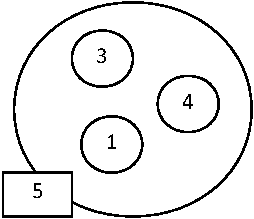
\includegraphics[]{Repraesentation2.pdf} 
      }
      \hspace{0.5cm}
      \subfigure[Tour 2]{
	\label{fig:Repraesentation3}
	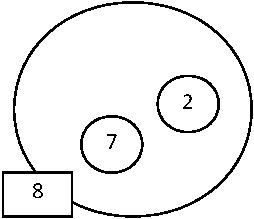
\includegraphics[]{Repraesentation3.pdf} 
      }
      \hspace{0.5cm}
      \subfigure[Tour 3]{
	\label{fig:Repraesentation4}
	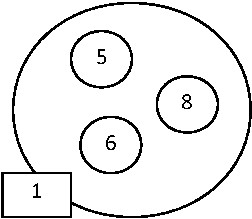
\includegraphics[]{Repraesentation4.pdf} 
      }
      \caption{Repräsentation Individuum (Plan)}
      \label{fig:Repraesentation234}
\end{figure}

Hierbei handelt es sich um ein konkretes Individuum, das drei Fahrzeuge verwendet, um die gezeigten acht Aufträge zu erfüllen. Zusätzlich muss jedes Gen mit einer ergänzenden Datenstruktur assoziiert werden, so dass im späteren Verlauf der Reihenfolgeaspekt dargestellt werden kann. Diese Darstellung wird im Umfeld des genetischen Algorithmus als Phänotyp bezeichnet. Dies veranschaulicht die \Fref{fig:Repraesentation5} zu einer gegebenen Tour:

\myfigure[]{Repraesentation5}{Repraesentation5.pdf}{Aktionsreihenfolge aus einem Gen}

Auf diese Informationen haben die genetischen Operatoren unmittelbaren Zugriff, um eine möglichst große Varianz in die spätere Population einzubringen.

\subsection{Aufbau der Startpopulation}
Bevor der genetische Algorithmus arbeiten kann, muss im ersten Schritt eine Startpopulation erzeugt werden, die für den Algorithmus als Ausgang dient. Dazu gibt es prinzipiell zwei verschiedene Vorgehensweisen:

\begin{enumerate}
 \item Zufällige Auswahl von Individuen mit zufälligen Merkmalen
 \item Auswahl von "`guten"' Individuen, die durch bestimmte Konstruktionsheuristiken erzeugt wurden
\end{enumerate}

Die zweite Variante bringt ein gewisses Risiko mit, da es beim genetischen Algorithmus passieren kann, dass die Suche, aufgrund bereits guter Lösungen, vorzeitigt konvergiert. Um diesem Problem entgegen zu wirken, wurde der Aufbau der Startpopulation mit beiden Möglichkeiten gekoppelt. Dies soll die  \Fref{fig:Repraesentation6} verdeutlichen:

\myfigure[]{Repraesentation6}{Repraesentation6.pdf}{Aufbau der Startpopulation}

Der Großteil der Population wird dabei zufällig erzeugt, wobei ein ausgewählter Teil sich den Konstruktionsheuristiken bedient. Dabei handelt es sich zum einen um das Nearest-Neighbor- und zum anderen um das Sweep-Verfahren, die in den folgenden Kapiteln kurz vorgestellt werden.

\subsubsection{Nearest-Neighbor}
Beim Nearest-Neighbor handelt es sich um ein bekanntes heuristisches Eröffnungsverfahren was beispielsweise zur Lösung des „Problems des Handlungsreisenden“ verwendet wird. Da das PDPTW eine Abwandlung von dieser Problemstellung ist, eignet sich diese Heuristik ideal für die Erzeugung von potentiellen Startindividuen. Dabei wird bei dieser Technik von einem beliebigen Startpunkt ausgehend der nächstdichteste Knoten besucht. Dies wird sukzessiv fortgesetzt, bis alle Knoten besucht wurden. 

\subsubsection{Sweep}
Der Sweep-Algorithmus bedient sich einer anderen Technik zum Finden des nächstmöglichen Knotens. Hier wird von einem beliebigen Knoten ausgehend, der Knoten gewählt, der den geringsten Winkel von einer definierten Startkante aufweist. Dies kann sowohl im oder entgegengesetzt dem Uhrzeigersinn durchgeführt werden.

\subsection{Individuenauswahl (Selektion)}
\label{sec:GenetischerSelektion}
Die Selektion bestimmt welche Individuen sich paaren dürfen, und erzeugt aus Ihnen die Menge der Nachkommen. Dabei kann die Auswahl entweder komplett zufällig stattfinden oder ins direkte Verhältnis zur Fitness eines Individuums gesetzt werden. Wenn man sich für eine reine fitnessproportionale Selektion entscheidet, so ist ein verhältnismäßig niedriger Selektionsdruck vorhanden, da der genetische Algorithmus verhältnismäßig lange konvergiert. Abhilfe schafft dort eine Ranglistenbasierte Selektion. Bei diesem Verfahren wird die Selektionswahrscheinlichkeit nicht mehr ins direkte Verhältnis zur Fitness gesetzt. Stattdessen werden die unterschiedlichen Individuen nach ihrer Fitness sortiert, so dass die Tour mit dem besten Ergebnis an oberster Stelle der Population steht. Im nächsten Schritt erfolgt die Auswahl der möglichen Kinder für die oberen Elemente der Rangliste mit einer höheren Wahrscheinlichkeit als tieferliegende Individuen. 

Zusätzlich wird auch hier auf ein Verfahren zurückgegriffen, welches die möglichen Eltern rein zufällig wählt. Dies hat den Vorteil, dass auch Individuen mit schlechter Fitness als potentieller Elternteil gewählt wird. Dadurch werden ggf. mehr genetische Informationen in die nächste Population übertragen und eine zu frühe Konvergenz, aufgrund von sehr guten Fitnesswerten, verhindert. 

Die Kombination der beiden Techniken veranschaulicht die \Fref{fig:Repraesentation7}. Dort wird als mögliches Elternpaar zum einen das Individuum 2 aufgrund der Fitness ausgewählt. Zum anderen wird Individuum 100 rein zufällig gewählt. Dadurch besteht der Vorteil, dass das Individuum, trotz schlechter Fitness, ggf. eine gute Kombination hervorbringt.

\myfigure[]{Repraesentation7}{Repraesentation7.pdf}{Individuenauswahl}

\subsection{Rekombination (Crossover)}
Bei der Rekombination, auch als Crossover bezeichnet, handelt es sich um den Vorgang, aus zwei Elternpaaren neue Individuen zu erzeugen. Dieses Verfahren stellt dabei einen der wichtigsten Suchoperatoren für genetische Algorithmen dar. Dabei werden die Nachkommen aus den Informationen der gekreuzten Elternpaare systematisch zusammengesetzt. Gesteuert wird der Crossover durch eine Wahrscheinlichkeit, die bestimmt ob entweder nur einfache Kopien der Eltern erzeugt werden, oder ein Operator zur Erzeugung der Nachkommen verwendet wird. Dazu werden nachfolgend zwei verschiedene Varianten vorgestellt.

\subsubsection{Crossover mit Control-String}
Bei dieser Variante der Rekombination wird, auf Grundlage der gewählten Eltern, ein Bit-String gebildet, der letztendlich zu der Entscheidung führt, ob sich der Nachkomme aus einem Teil des ersten oder zweiten Elternteils zusammensetzt. Im Kontext der Fahrzeugeinsatzplanung soll dies die \Fref{tab:CrossoverControlString} verdeutlichen:

\begin{table}[ht!]
 \centering
 \caption{Crossover mit Control-String}
 \begin{tabular}{ll}
  \textbf{Fahrzeug 1 (Plan 1):}	& $1+ \rightarrow 4+ \rightarrow 1- \rightarrow 7+ \rightarrow 7- \rightarrow 4-$ \\
  \textbf{Control-String:} 	& 1 ~ 0 ~ 0 ~ 0 ~ 1 ~ 1 ~ 0 ~ 1 ~ 0 ~ 1 \\
  \textbf{Fahrzeug 1 (Plan 2):} 	& $1+ \rightarrow 5+ \rightarrow 5- \rightarrow 1-$ \\
  \textbf{Nachkomme:} 		& $1+ \rightarrow 5+ \rightarrow 5- \rightarrow 1- \rightarrow 4+ \rightarrow 7+ \rightarrow 7- \rightarrow 4-$
 \end{tabular}
 \label{tab:CrossoverControlString}
\end{table}

Oben und unten ist jeweils eine Tour dargestellt, die jeweils einem Elternindividuum entnommen wurde. In der Mitte befindet sich der "`Control-String"', wobei die Länge der Summe der Aufträge (Be- und Entladung) der beiden Eltern entspricht. Nun nimmt ein Element des Strings zufällig eine Ausprägung von "`1"' oder "`0"' an, wobei die "`1"' besagt, dass das Element aus Fahrzeug 1 von Plan 1 für den Nachkommen gewählt wird. Auf gleiche Weise geschieht dies mit der "`0"' für Fahrzeug 1 aus Plan 2. Bereits gewählte Aufträge werden dabei nicht mehr berücksichtigt. Letztendlich entsteht der unten in der \Fref{tab:CrossoverControlString} aufgeführte Nachkomme.

\subsubsection{Crossover nach Falkenauer}
Die zweite Variante für einen möglichen Crossover orientiert sich an dem gruppenzentrierten Operator, der von Falkenauer vorgeschlagen wurde. Im Wesentlichen besteht er aus vier Phasen die nachfolgend in der \Fref{fig:CrossoverFalkenau} dargestellt und erläutert werden.

\myfigure[width=0.9\textwidth]{CrossoverFalkenau}{CrossoverFalkenau.png}{CrossOver nach Falkenauer \cite{bortfeldtplanen}}

\begin{enumerate}
 \item In der ersten Phase werden in jedem der beiden Eltern zufällig je zwei Crossover-Punkte gebildet, die innerhalb von jedem Elternteil den Anfang und das Ende des Crossover-Segments darstellen.
 \item Hier wird das Crossover-Segment des zweiten Elternteils an den ersten Crossover-Punkt des ersten Elternteils angefügt. Die dazugehörigen Touren werden vom Elternteil unmittelbar übernommen, also vorerst ohne Neukonstruktion. Als Folge kann eine Anzahl von Aufträgen mehreren Fahrzeugeinsatzplänen zugeordnet sein. Desweiteren kann es auch vorkommen, dass mehrere Touren vom gleichen Fahrzeug bedient werden.
 \item In dieser Phase werden alle auftretenden Probleme aus Punkt 2 aufgelöst. Dabei wird so vorgegangen, dass vorerst alle neuerhaltenden Touren unangetastet bleiben und die Touren des empfangenden Elternteils modifiziert werden, um alle Konflikte zu lösen. Dazu werden alle Touren eliminiert, die auf ein Fahrzeug referenzieren, das neu hinzugefügt wurde (im Beispiel Fahrzeug 1). Falls anschließend noch einzelne Aufträge doppelt vorhanden sind, so werden auch diese aus den Touren des empfangenden Elternteils eliminiert (im Beispiel die Aufträge 2, 6 und 7). Nach Abschluss dieser Operation sind einzelne Aufträge (im Beispiel 5 und 8) noch vorerst keiner Tour zugeordnet.
 \item Die verbleibenden Aufträge werden rein zufällig an die vorhandenen Touren vergeben. Dazu kann beispielsweise auch ein komplett neues Fahrzeug allokiert werden. Nach Abschluss von Schritt 4 liegt letztendlich als Ergebnis ein vollständiges Kind vor.
\end{enumerate}

Gegebenenfalls können die Schritte 2-4 mit vertauschten Rollen der Eltern wiederholt werden, falls man ein zweites Kind erzeugen möchte.

\subsection{Mutation}
Unter der Mutation, im Zusammenhang zum Genetischen Algorithmus, versteht man die Art und Weise, um aus einem Elternteil ein neues Individuum durch zufällige Veränderung zu erzeugen. Diese Änderung wird dabei auch hier durch eine Wahrscheinlichkeit gesteuert, die angibt, ob eine Mutation an einem Individuum stattfindet oder nicht. Sie dienen hauptsächlich dazu, eine gewisse Inhomogenität und Divergenz mit in die Population herein zu bringen, was durch die Rekombination unter Umständen nicht möglich ist. Zusätzlich wird eine frühzeitige Konvergenz des Algorithmus verhindert und der Selektionsdruck abgeschwächt. 

Innerhalb dieser Arbeit wurden insgesamt sieben verschiedene Mutationsoperatoren entwickelt, welche mit einer Gewichtung dem genetischen Algorithmus hinzugefügt werden können. Diese werden im nachfolgenden jeweils mit einer Abbildung vorgestellt.

\subsubsection{Aufteilung der längsten Route}
\label{sec:AufteilungLangaesteRoute}
Dieser Operator überprüft die Länge von jeder Tour innerhalb einer Fahrzeugeinsatzplanung. Die Tour, welche die längste Strecke anhand der gefahrenen Kilometer aufweist (im Beispiel Fahrzeug 5), wird entfernt und auf die verbleibenden Touren aufgeteilt (siehe \Fref{fig:MutationAufteilen1} und \Fref{fig:MutationAufteilen2}). Dabei werden die Aufträge rein zufällig an die anderen Touren vergeben.

\myfigure{MutationAufteilen1}{MutationAufteilen1.pdf}{Ausgangsindividuum}
\myfigure{MutationAufteilen2}{MutationAufteilen2.pdf}{Neues Individuum}

\subsubsection{Aufteilung der kleinsten/zufälligen Tour}
Diese beiden Mutationsoperatoren arbeiten auf die gleiche Weise wie unter \Fref{sec:AufteilungLangaesteRoute} beschrieben. Dabei wird hier der mögliche Kandidat entweder zufällig oder anhand der kleinsten Tour gewählt. Da die Arbeitsweise nahezu identisch ist, wurde hier auf eine zusätzliche Abbildung verzichtet.

\subsubsection{Verschiebung einer/mehrerer Aktion(en) innerhalb einer Tour}
Dieser Operator geht noch einen Schritt weiter und verschiebt innerhalb einer Tour eine Aktion. Bei einer Aktion kann es sich um ein Auf- oder Abladen eines bestimmten Auftrags handeln, was über die assoziierte Datenstruktur zu einer Tour gewährleistet wird. (siehe \Fref{fig:AktionVerschieben}). Ein weiterer Operator verschiebt zusätzlich nicht nur eine Aktion, sondern ganze Subrouten, die in ihren Grenzen zufällig gewählt werden.

\myfigure[]{AktionVerschieben}{AktionVerschieben.pdf}{Verschiebung einer/mehrerer Aktion(en) innerhalb einer Tour}

Die Repräsentation (links in \Fref{fig:AktionVerschieben}) bleibt davon unberührt, da es sich um eine reine Manipulation der Datenstruktur handelt. Konkret wird in diesem Beispiel das Abladen des Auftrags 3 mit dem Aufladen des Auftrags 2 vertauscht. Dies kann zur Folge habe, dass falsche Lösungen entstehen, da nach dem Operator keine Überprüfung und ggf. eine Korrektur stattfindet. Der Umgang mit der genannten Problematik wird jedoch im \Fref{sec:Nachfolgegeneration} erläutert. 

\subsubsection{Verschiebung von Subtouren über eine Tour hinaus}
Die bisherigen Operatoren haben lediglich ein Gen des Individuums mutiert. Um eine größere Varianz, unter dem Einfluss der Mutation, zu erschaffen wurde zusätzlich eine Möglichkeit entwickelt, wo ein Tauschen von Subtouren zwischen den unterschiedlichen Genen eines Individuums stattfindet. Dies veranschaulicht die \Fref{fig:SubrouteVerschieben}:

\myfigure[]{SubrouteVerschieben}{SubrouteVerschieben.pdf}{Verschiebung von Subtouren über eine Tour hinaus}

Dadurch entstehen letztendlich zwei komplett neue Touren innerhalb einer Fahrzeugeinsatzplanung, wobei diese Mutation Einfluss auf die Repräsentationsebene hat, da beispielsweise die Order 2 und 7 von Tour 2 nun von der Tour 1 ausgeführt wird. 

\subsubsection{Kombination von 2 Touren}
Den letzten genetischen Operator für eine Mutation stellt die Kombination von 2 Touren zu einer neuen Tour dar. Das Fahrzeug, das die Aufträge abliefert, wird zufällig aus den beiden vorhandenen gewählt. Dies wird durch die \Fref{fig:Kombination} veranschaulicht:

\myfigure[]{Kombination}{Kombination.pdf}{Kombination von zwei Touren}

\FloatBarrier
~\newpage
\subsection{Fitnesstest}
\label{sec:Fitnesstest}
Um die Individuen einer Population bewerten zu können, werden sie einem Fitnesstest unterzogen. Der hierbei ermittelte Fitnesswert gibt dann Aufschluss über die Qualität eines Individuums. In der Fahrzeugeinsatzplanung ist die Qualität eines Plans von verschiedenen Komponenten abhängig, beispielsweise von der Länge, von der Anzahl der verwendeten Fahrzeuge oder von der Art und Anzahl der Restriktionsverletzungen. Der in diesem Projekt verwendete Fitnesstest ist modular aufgebaut und sieht für die unterschiedlichen Komponenten jeweils einen separaten Baustein vor. Folgende Bausteine sind in der Applikation vorhanden:
\begin{itemize}
 \item Länge eines Plans ({\slshape{LengthFitnessTest}})
 \item die Anzahl der verwendeten Fahrzeuge für einen Plan ({\slshape{VehicleFitnessTest}})
 \item Verletzung der Kapazitätsbedingungen ({\slshape{CapacityFitnessTest}})
 \item Verletzung der Zeitfenster der Fahrzeuge ({\slshape{VehicleMakeSpanFitnessTest}})
 \item Verletzung der Zeitfenster der Aufträge ({\slshape{LoadingFitnessTest}})
\end{itemize}
Je nach Wunsch der Optimierung können diese Bausteine dann zusammengesetzt werden. Hierbei sind alle Kombinationen der genannten Bausteine möglich, auch die Verwendung eines einzelnen Bausteins ist vorgesehen.

Jeder Baustein berechnet hierbei seinen eignen Fitnesswert und je nach Zusammensetzung des Fitnesstests werden diese dann addiert. Ziel ist es die Summe der einzelnen Fitnesswerte zu minimieren. Die Problematik beim Berechnen der Gesamtfitness besteht darin, dass unterschiedliche Einheiten verwendet werden, zum Beispiel Mengenangaben für die Anzahl der Fahrzeuge oder Zeitangaben für Verletzungen der Zeitfenster. Deshalb wird als Basis für die jeweiligen Fitnesswerte die Länge eines Plans verwendet. Je nach Baustein wird die Länge dann mit einem bestimmten Faktor multipliziert. Dieser Faktor ergibt sich aus der Wichtigkeit eines Bausteins und aus einem spezifischen Wert, beispielsweise die Anzahl der verwendeten Fahrzeuge. Die Wichtigkeit eines Bausteins kann von außen angegeben werden. Dadurch ist es einem Anwender möglich, festzulegen welche Komponenten für ihn wichtig sind, zum Beispiel möchte Anwender A die kürzeste Strecke zurücklegen und nimmt dafür Verletzungen der Zeitfenster in Kauf, dagegen möchte Anwender B unbedingt alle Restriktionen einhalten und akzeptiert einen längeren Weg.

Eine Besonderheit bei diesem Fitnesstest stellen die Bausteine mit den Restriktionsverletzungen dar. Bei diesen Bausteinen wird folgendes Verhalten umgesetzt: mehrere kleine Verletzungen sind nicht so schlimm wie eine große, beispielsweise ist die Qualität eines Plans besser, wenn zwei Fahrzeuge um jeweils eine halbe Stunde ihr Zeitfenster verfehlen als wenn ein Fahrzeug um eine Stunde sein Zeitfenster verfehlt. Dafür wird eine exponentielle Bestrafung eingesetzt.

\subsection{Bildung der Nachfolgegeneration}
\label{sec:Nachfolgegeneration}
Über die Mechanismen der Selektion hinaus, die in \Fref{sec:GenetischerSelektion} definiert wurden, wird sowohl die komplette Ausgangspopulation, als auch die neue Population, für die Nachfolgepopulation berücksichtigt. Dazu findet auch an der Neuen wiederum eine Sortierung statt. Zum einen werden alle invaliden Lösungen, d.h. Lösungen, wo beispielsweise ein Ent- vor dem Beladen erfolgt, ans Ende der Population verschoben. Danach erfolgt eine Sortierung anhand der Fitness. Demnach werden beiden Populationen zu einer Nachfolgepopulation der definierten Menge (im Beispiel 100) zusammengefasst. Zur Veranschaulichung dient die \Fref{fig:Nachfolgegeneration}:

\myfigure[scale=0.85]{Nachfolgegeneration}{Nachfolgegeneration.pdf}{Bildung der Nachfolgegeneration}

Das Resultat ist die neue Nachfolgepopulation, die wieder in den genetischen Algorithmus einfließt, bis eine Abbruchbedingung erreicht wird. Diese Verfahrenstechnik hat den Vorteil, dass bereits potentiell gute Lösungen, die in der Ausgangspopulation vorhanden waren, erhalten bleiben und nicht durch die neugebildete Population überschrieben werden.

\FloatBarrier
\subsection{Abbruchbedingung}
Als letzten entscheidenden Punkt muss beim genetischen Algorithmus eine Abbruchbedingung definiert werden, wann die Suche abgeschlossen ist. Dazu wurden zwei Varianten entwickelt:

\begin{enumerate}
 \item Der genetische Algorithmus wird solange durchlaufen, bis eine definierte Anzahl von Iterationen (z.B. 5000) erreicht wurde.
 \item Die Fitness der besten Lösung entspricht einem definierten Abstand von der Durchschnittsfitness von allen Lösungen zu dieser Lösung
\end{enumerate}

Die erste Bedingung wird für den Fall benötigt, dass der genetische Algorithmus nicht unendlich oft durchlaufen wird. Eine Iteration entspricht dabei dem Weg von einer Ausgangspopulation bis hin zu Neubildung der Nachfolgegeneration.

Die zweite Bedingung ist die eigentlich entscheidende, da der Algorithmus solange laufen soll, bis keine bessere Lösung mehr gefunden wird. Ist dies der Fall, so kann die genetische Suche abgeschlossen werden und das erste Individuum in der Population entspricht der optimalen Lösung für eine gegebene Konfiguration.
